\documentclass{beamer}
\usepackage{graphicx}


\usetheme{simple}

\usepackage{lmodern}
\usepackage[scale=2]{ccicons}

% TODO: 
%   position adjustement
%   change colours
%       

% Watermark background (simple theme)

% \setwatermark{
\includegraphics[height=8cm]{img/uwat.jpg}}
\setwatermark{\fontsize{125pt}{125pt}\selectfont{Overfit}}


\newcommand{\heart}{\ensuremath\heartsuit}

\title{Melbourne University AES/MathWorks/NIH Seizure Prediction}
\subtitle{}
\date{\today}
\author{Shivam Kalra \& Ruifan Yu \\ \texttt{\{shivam.kalra,ruifan.yu\}@uwaterloo.ca}}

\institute{}

\begin{document}

\maketitle

\begin{frame}{Problem Description}
  \framesubtitle{Introduction}

  \begin{itemize}
  \item
    Nearly one-third of patients with epilepsy continue to have \textbf{seizures} despite
    optimal medication management \cite{ramgopal_seizure_2014}.

  \item
    Seizures are a symptom associated with abnormal electrical activity in the
    brain.

  \item
    \alert{What is a seizure?} and \alert{When to detect it?} questions remain
    elusive.

  \item
    Plenty data is available, \textbf{machine learning} can help in building
    seizure forecasting systems.

  \item
     \textbf{Could save life!}
    
  \end{itemize}

\end{frame}

\begin{frame}{Problem Description}
  \framesubtitle{Melbourne University AES/MathWorks/NIH Seizure Prediction}
  \begin{block}{What is given and what is required?}
    \begin{itemize}
    \item
      Human brain activity (intracranial EEG) taken from multiple sensors on
      brain.

    \item
      Each recording is \textbf{10 minutes} long, recorded at \textbf{400 Hz}
      resulting $\boldsymbol{240,000}$ data points per recording.

    \item
      Challenge is to classify unseen recording as \textbf{Preictal}
      (prior to seizure) or \textbf{Interictal} (at least an hour before
      seizure).
    \end{itemize}
  \end{block}
    
\end{frame}

\begin{frame}{Problem Description}
  \framesubtitle{Tell me if this is Interictal or Preictal?}
  \begin{columns}
    \column{0.5\textwidth}
    \hspace*{-0.9cm}
    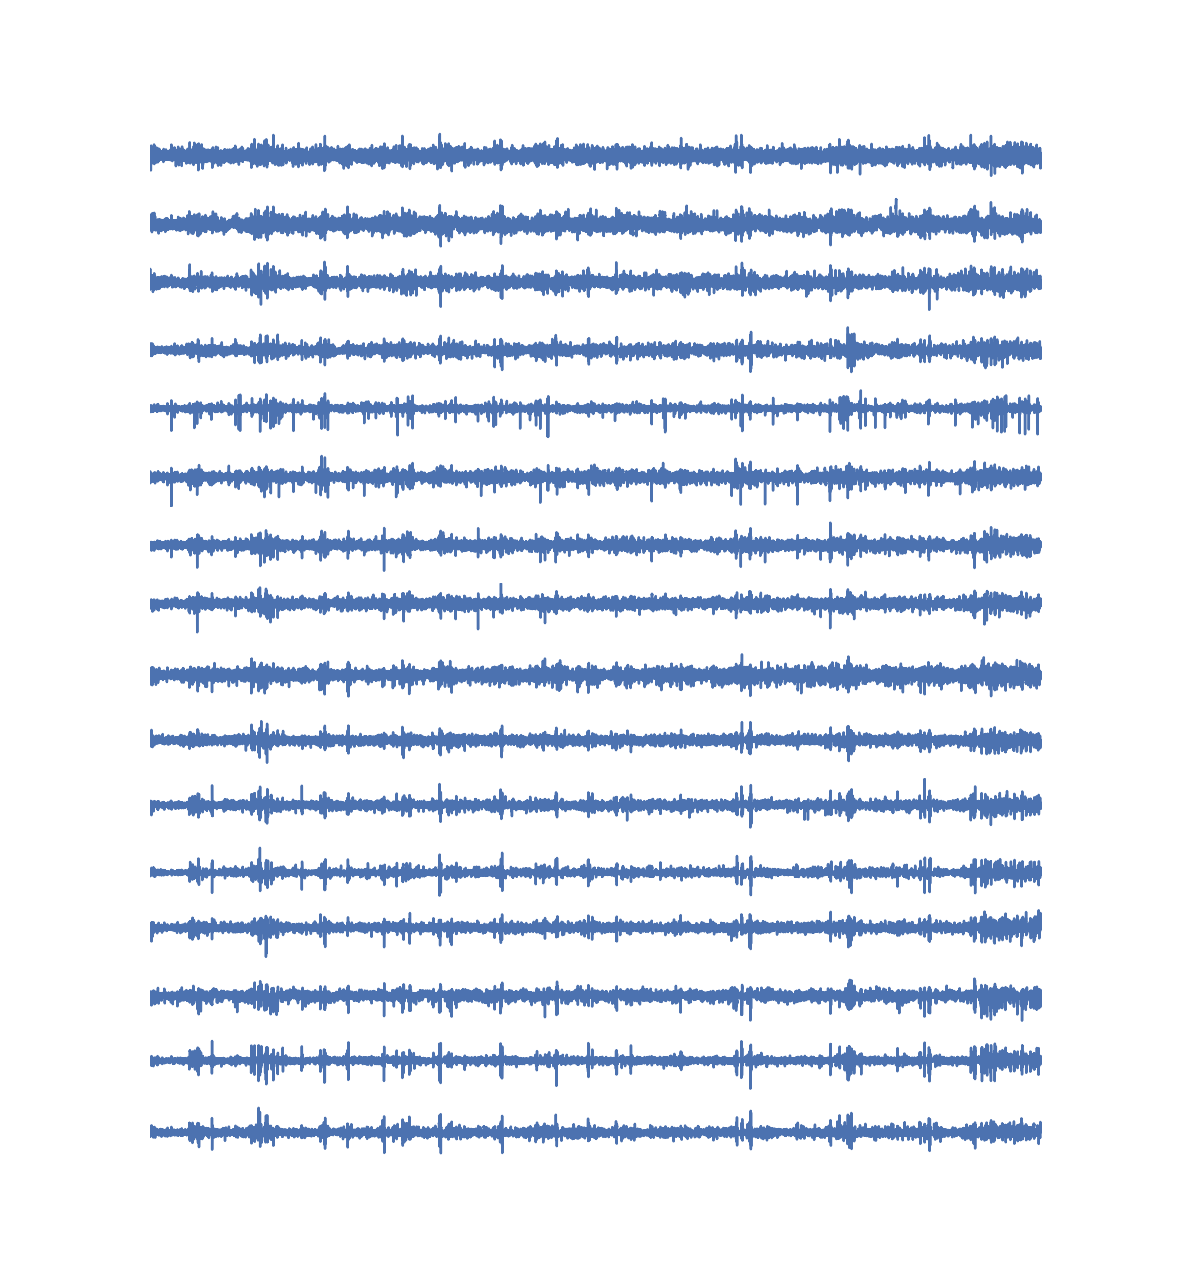
\includegraphics[scale=0.25]{img/all_data.eps}
    \column{0.4\textwidth}
    \begin{block}{Input}
      Figure shows \textbf{one sample of input data} from Patient 1's data-set.
      Shape of the data is $16 \times 240000$.
    \end{block}

    \begin{block}{Output}
      Classifier model needs to figure out if it is \textbf{Preictal} or
      \textbf{Interictal}.
    \end{block}

  \end{columns}
\end{frame}

\begin{frame}{Problem Description}
  \framesubtitle{Red is Preictal. But predicting this is not very trivial...}
  
  \begin{columns}
    \column{0.4\textwidth}
    \includegraphics[scale=0.23]{img/iex.eps}
    \column{0.5\textwidth}
    \includegraphics[scale=0.23]{img/pex.eps}

  \end{columns}
\end{frame}


\begin{frame}{Problem Description}
  \framesubtitle{How good is raw data?? TSNE visualization for Patient 1 Channel 3.}
  \begin{center}
    \vspace*{-0.5cm}
    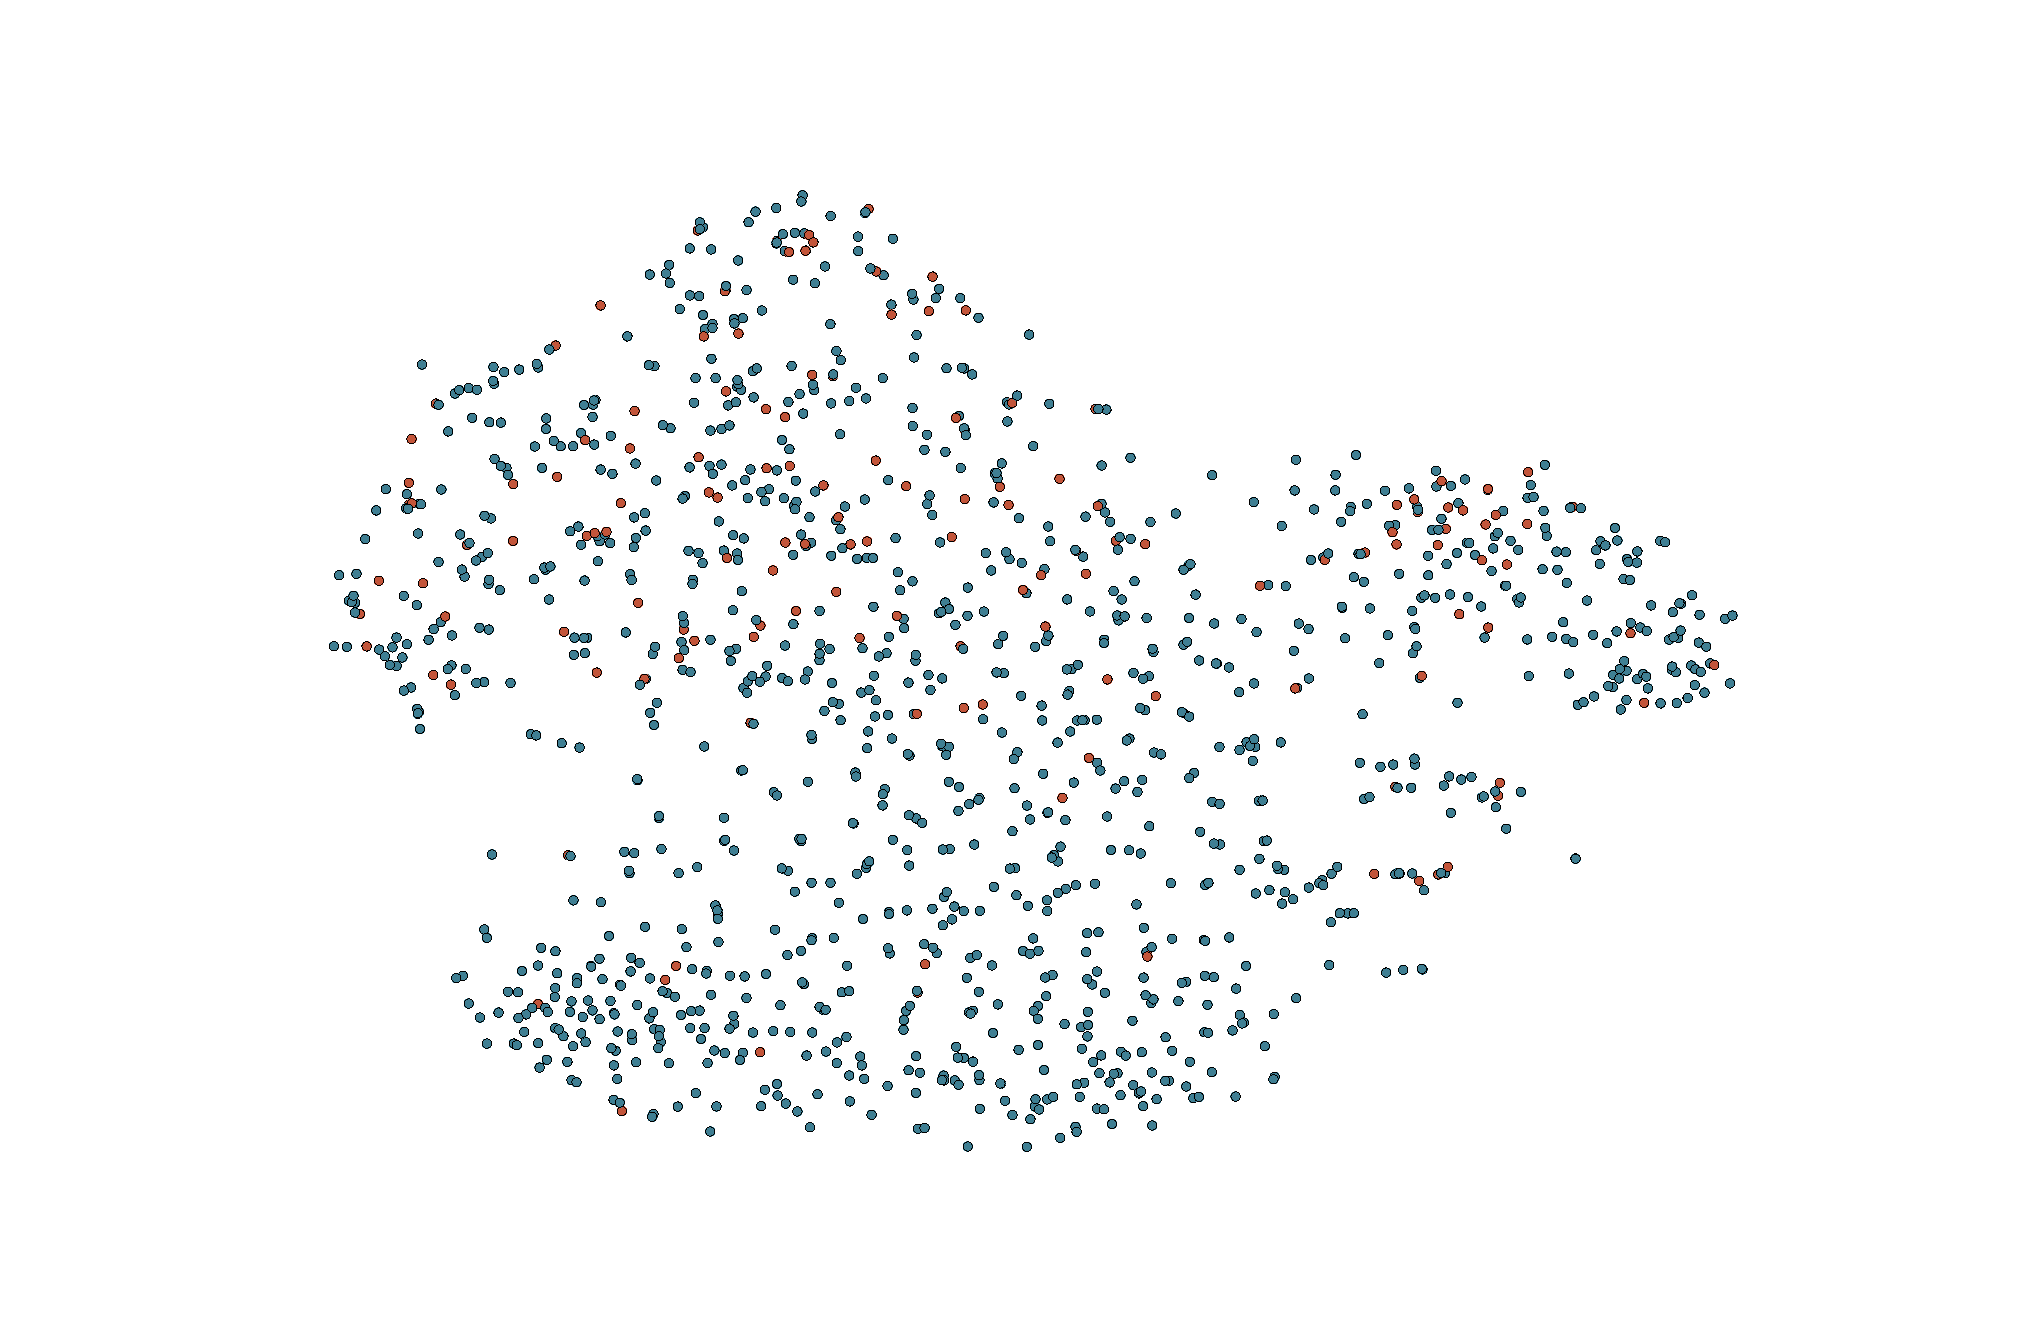
\includegraphics[scale=0.32]{img/tsne_raw_data.eps}
  \end{center}
\end{frame}

\begin{frame}{Problem Description}
  \framesubtitle{Okay, so prediction is hard on raw data..but we got more issues!!!}

  \begin{columns}
    \column{0.35\textwidth}
    
\includegraphics[scale=0.38]{img/serious.jpg}
    \column{0.45\textwidth}
    \begin{block}{}
      Apart from being already difficult prediction problem, we got bigger
      issues with data-set. \textbf{This is not cool!!}
    \end{block}
  \end{columns}
\end{frame}


\begin{frame}{Problems with Data Set}
  \framesubtitle{There are only two types of people in the world, those who can
    extrapolate from incomplete data...}

  \begin{columns}
    
    \column{0.5\textwidth}
      % 
\includegraphics[scale=0.43]{img/baddata.jpg}
      
\includegraphics[scale=0.35]{img/data_problems.png}

    \column{0.4\textwidth}

    \begin{block}{Training Data-set has...}
      \begin{enumerate}
      \item Categorical Imbalance
      \item Missing Data or Random Dropouts
      \end{enumerate}
    \end{block}

  \end{columns}
  
\end{frame}

\begin{frame}{Problems with Data Set}
  \framesubtitle{Categorical Imbalance}

  \begin{center}
    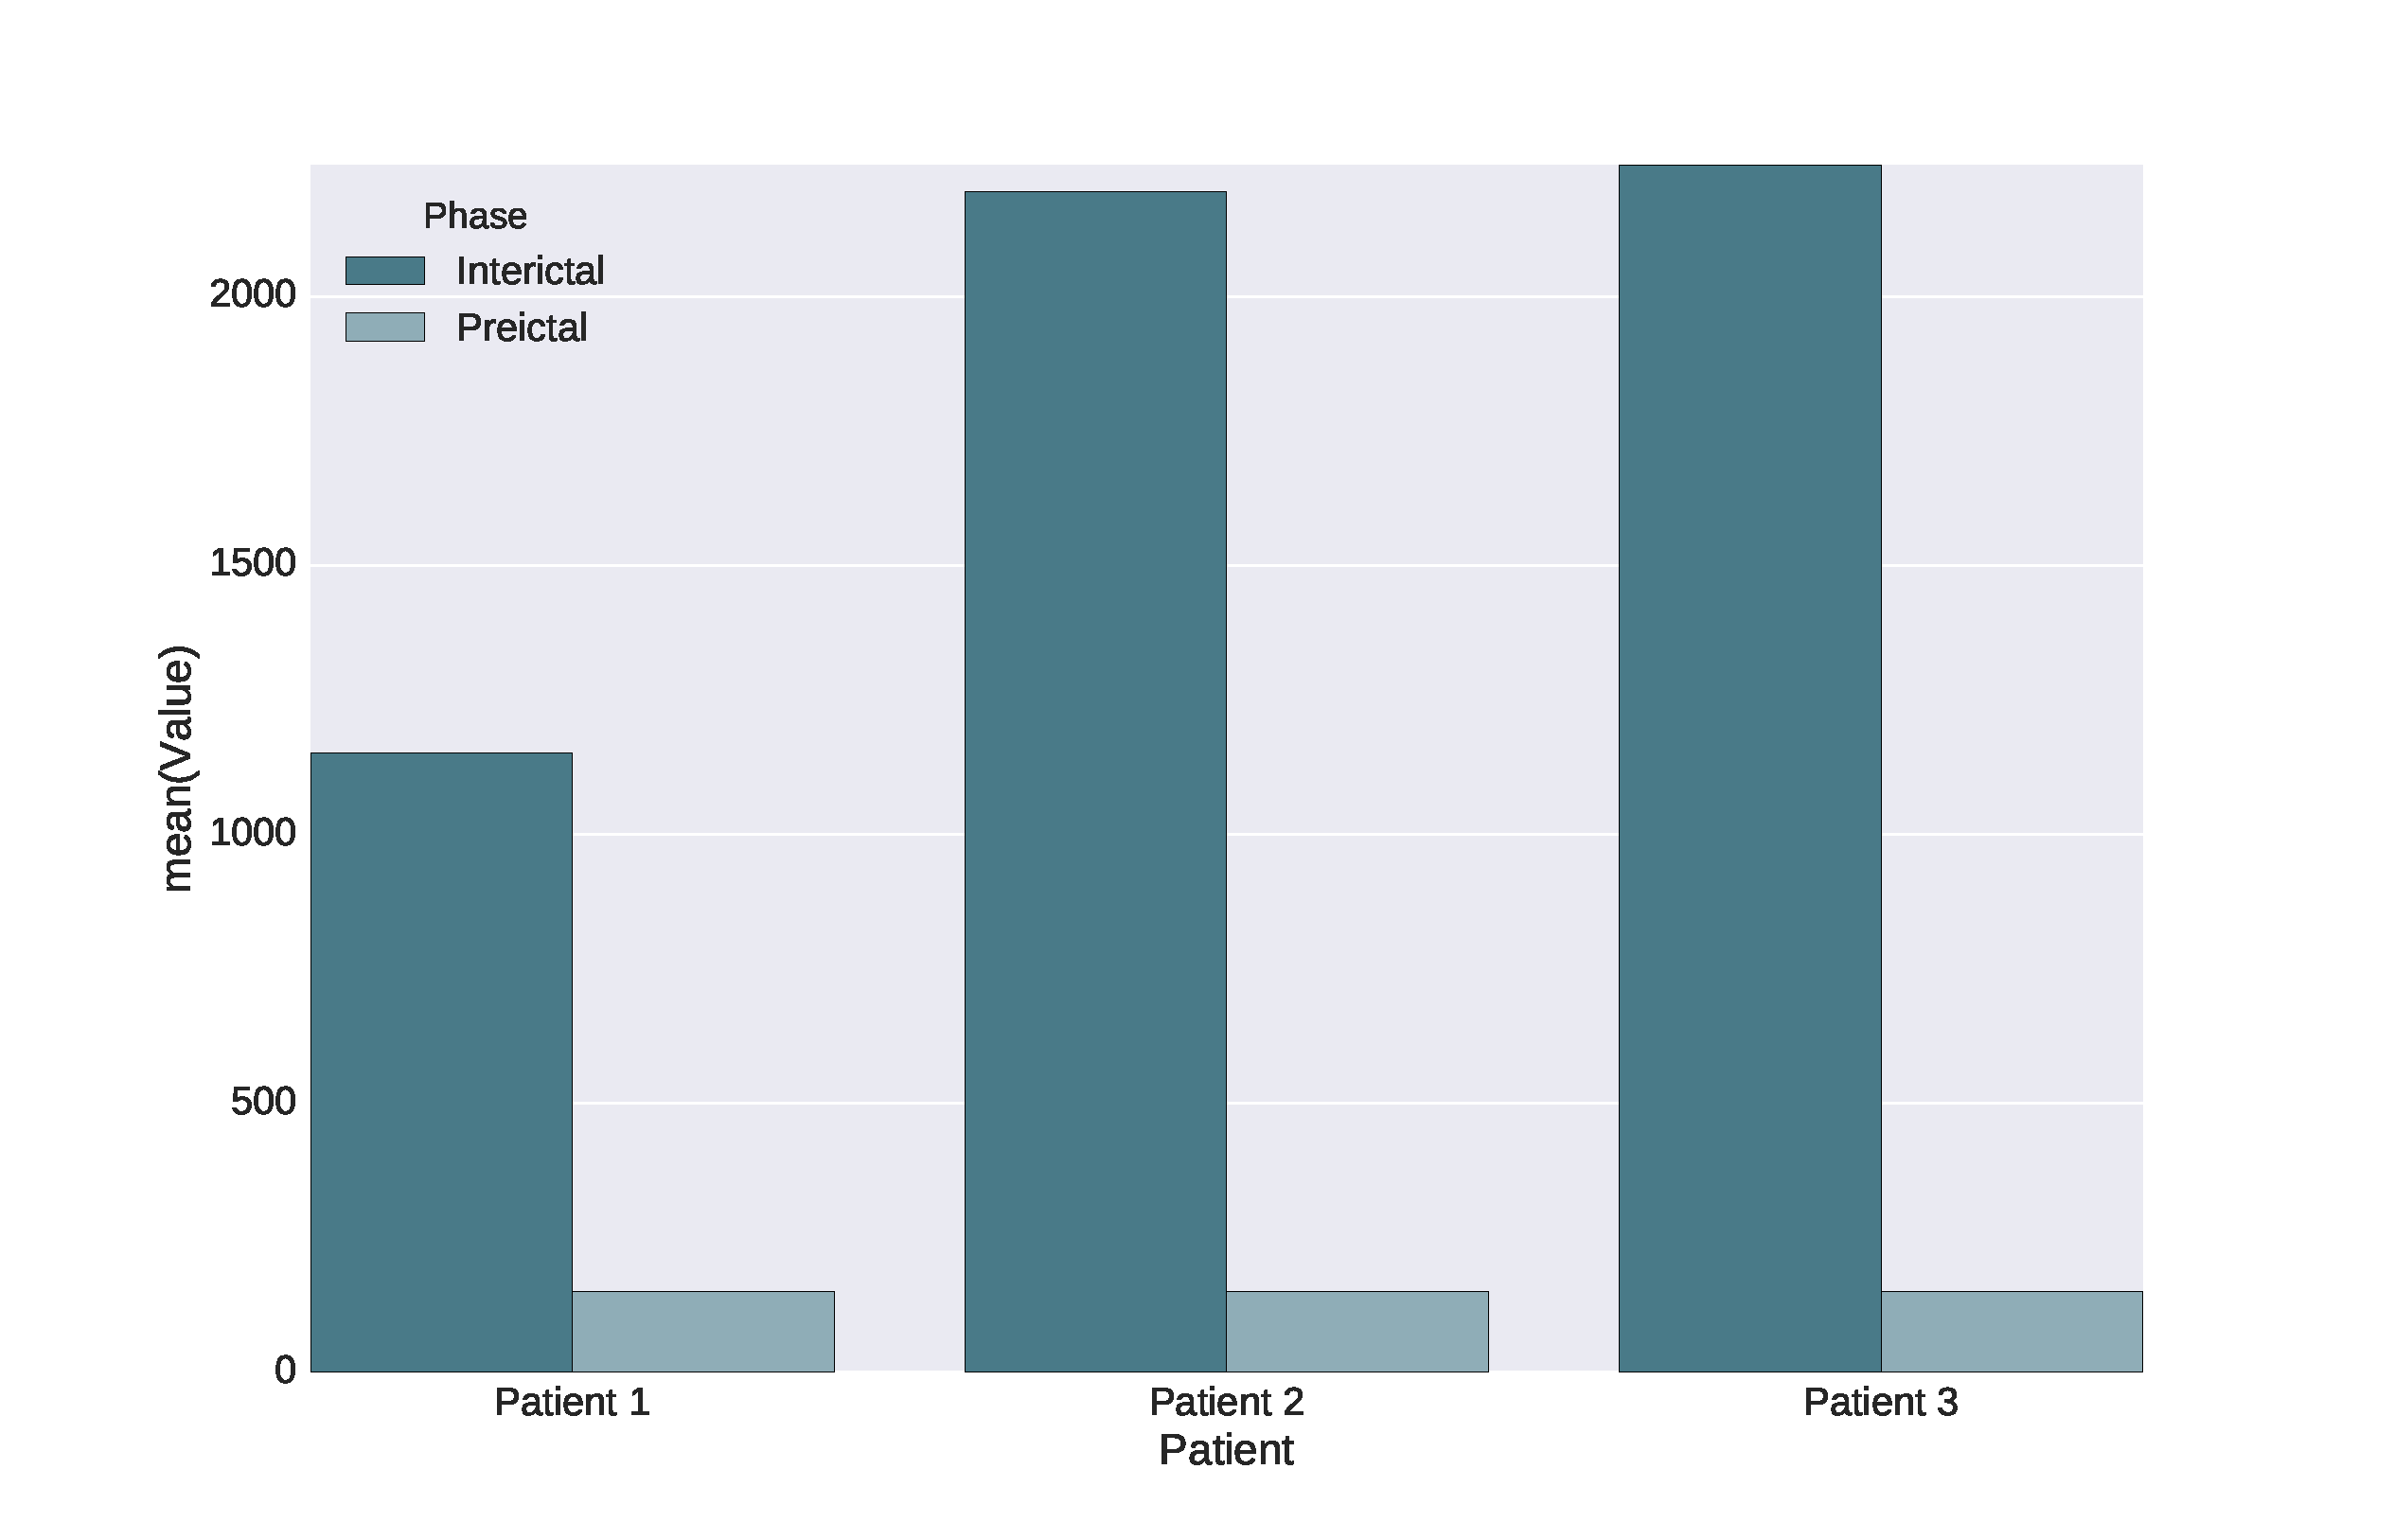
\includegraphics[scale=0.28]{img/cat_imbalance.eps}
  \end{center}
\end{frame}


\begin{frame}{Problems with Data Set}
  \framesubtitle{Missing/Dropouts in Data Set}

  \begin{block}{}
    \begin{itemize}
    \item Random dropouts of \textbf{10 seconds or more} in the EEG signals across all the 16 channels.
    \item Exist in \textbf{abundance} (even in testing data set).
    \item Some training data is \textbf{entirely empty} (completely missing!!!)
    \end{itemize}
  \end{block}

  \begin{columns}
    \column{0.55\textwidth}
    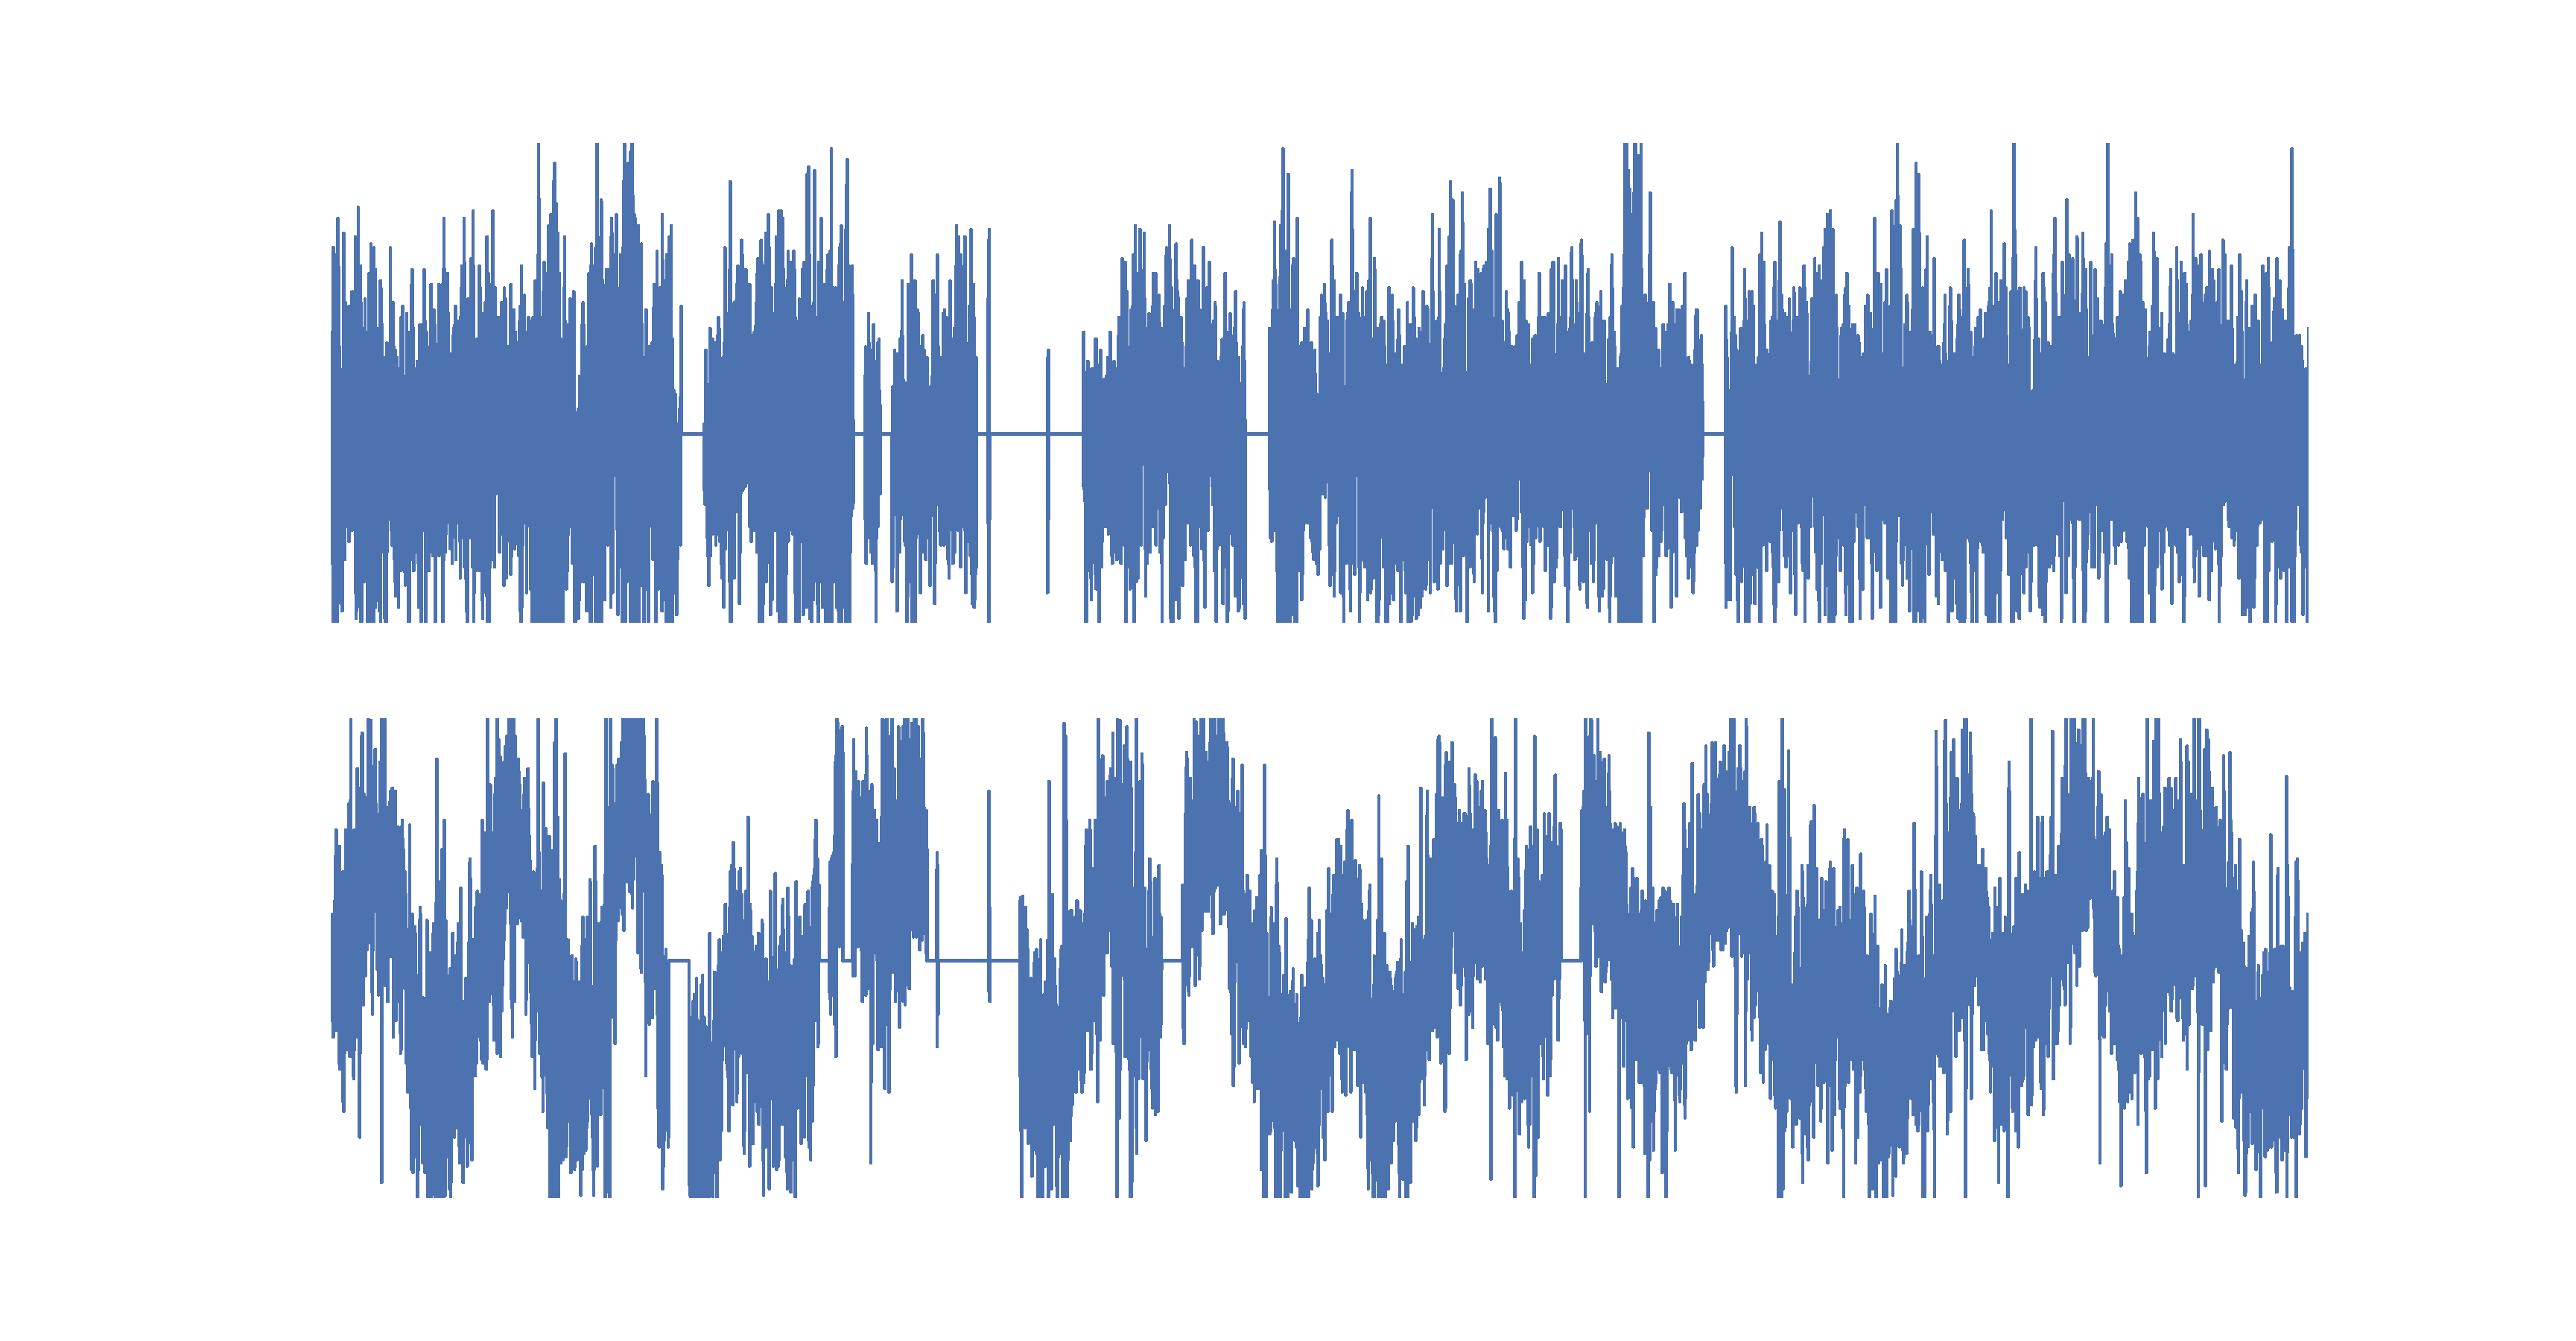
\includegraphics[scale=0.13]{img/data_drops2.eps}

    \column{0.37\textwidth}
    \textbf{Figure: Missing data in channel 1 and 3 from Patient 1's data set}
  \end{columns}
\end{frame}

\begin{frame}{Classification}
  \framesubtitle{Ingredients of our present classifier...}

  \textbf{Ensemble} of 3 different classifier models:
  
  \begin{enumerate}
  \item \textbf{Deep Learning:} CNN classification of Spectrograms
  \item SVM classification on \textbf{Random Transforms} of Spectrograms
  \item SVM/LR/RF  classification using various \textbf{DSP features}
  \end{enumerate}

  \pause
  \begin{block}{Kaggle score}
    We are at AUC $\boldsymbol{\sim 0.74}$ as of now.
  \end{block}
\end{frame}


\begin{frame}{Model 1: Deep Learning (CNN) on Spectrograms}
  \framesubtitle{}
  \begin{columns}
    \column{0.38\textwidth}
  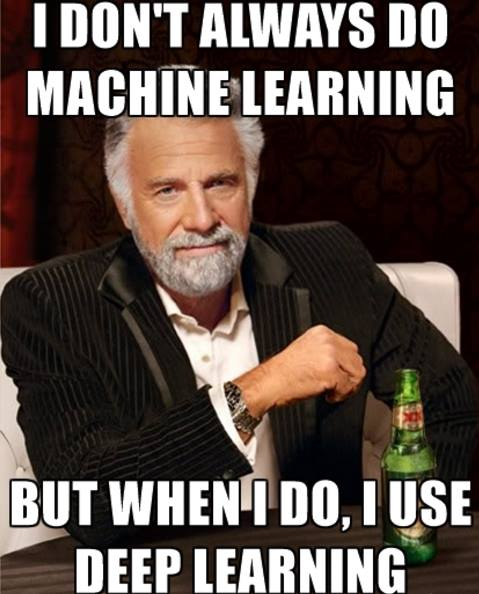
\includegraphics[scale=0.27]{img/deep.png}
    \column{0.55\textwidth}
    
\includegraphics[scale=0.18]{img/deeper.jpg}
  \end{columns}
\end{frame}


\begin{frame}{Model 1: Deep Learning (CNN) on Spectrograms}
  \framesubtitle{Some background research...}

  \begin{block}{Why Convolution Neural Networks?}
    \begin{itemize}
    \item Our \textbf{eternal love} for deep learning...
    \item Successful results by CNN in seizure detection as in
      ~\cite{korshunova_faculty_2015,mirowski2008comparing}.
    \item Iryna Korshunova's CNN approach in~\cite{korshunova_faculty_2015}
      topped among best $10\%$ in 2014's seizure prediction competition.
    \end{itemize}
  \end{block}
\end{frame}


\begin{frame}{Model 1: Deep Learning (CNN) on Spectrograms}
  \framesubtitle{And the most important reason we choose deep learning...}
  
  \begin{block}{\texttt{deepfit}..who are they? Sounds deep learn*ish*!!}
    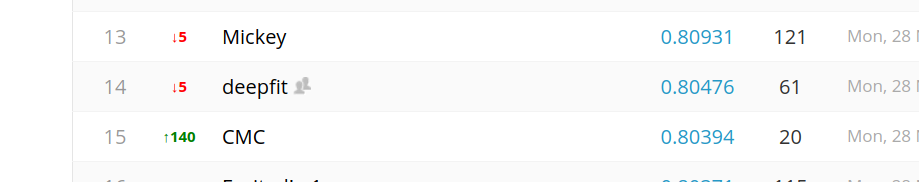
\includegraphics[scale=0.3]{img/who_are_they.png}
  \end{block}


  \begin{itemize}
  \item This is some \textbf{random team on leader board} (not from this class most likely??).
  \item Another motivation to pursue \textbf{deep learning}.
    \pause
  \item \textbf{However, they may not be using deep learning..we don't know yet!!}

  \end{itemize}

\end{frame}

\begin{frame}{Model 1: Deep Learning (CNN) on Spectrograms}
  \framesubtitle{Input/Output for training of CNN...}

  \begin{block}{Preprocessing}
    All the \textbf{unsafe} is removed as per guideline of competition.
  \end{block}
  
  \begin{block}{Input}
    \begin{itemize}
    \item Raw wave data is converted into \textbf{Spectrograms}.
    \item \textbf{Frequencies} are binned into \textbf{6 bands}.
    \item \textbf{Time domain} is binned with windows of \textbf{20 seconds} each.
    \end{itemize}
  \end{block}  

  \begin{block}{Output}
    \begin{itemize}
      \item Interictal $[1, 0]$
      \item or, Preictal   $[0, 1]$
    \end{itemize}
  \end{block}  

\end{frame}

\begin{frame}{Model 1: Deep Learning (CNN) on Spectrograms}
  \framesubtitle{Frequency bands in Spectrograms}

  Frequency bands are chosen as in~\cite{korshunova_faculty_2015}.
  
  \begin{block}{}
    \begin{table}[]
      \centering
      \caption{Frequency bands in Spectrograms}
      \begin{tabular}{ll}
        \textbf{Name}               & \textbf{Frequency Range (Hz)} \\
        \textbf{Delta}     & 0.4 -- 4                      \\
        \textbf{Theta}     & 4 -- 8                        \\
        \textbf{Alpha}     & 8 -- 12                       \\
        \textbf{Beta}      & 12 -- 30                      \\
        \textbf{Lowgamma}  & 30 -- 80                      \\
        \textbf{Highgamma} & 80 -- 180                    
      \end{tabular}
    \end{table}
  \end{block}

\end{frame}

\begin{frame}{Model 1: Deep Learning (CNN) on Spectrograms}
  \framesubtitle{Final Spectrogram as Input to CNN}

  Final Spectrogram becomes: $16 \times 6 \times 10$. \textbf{Right is Preictal,
    can you guess? Well, lets leave it to CNN to classify!}

  \begin{columns}
    \column{0.5\textwidth}
    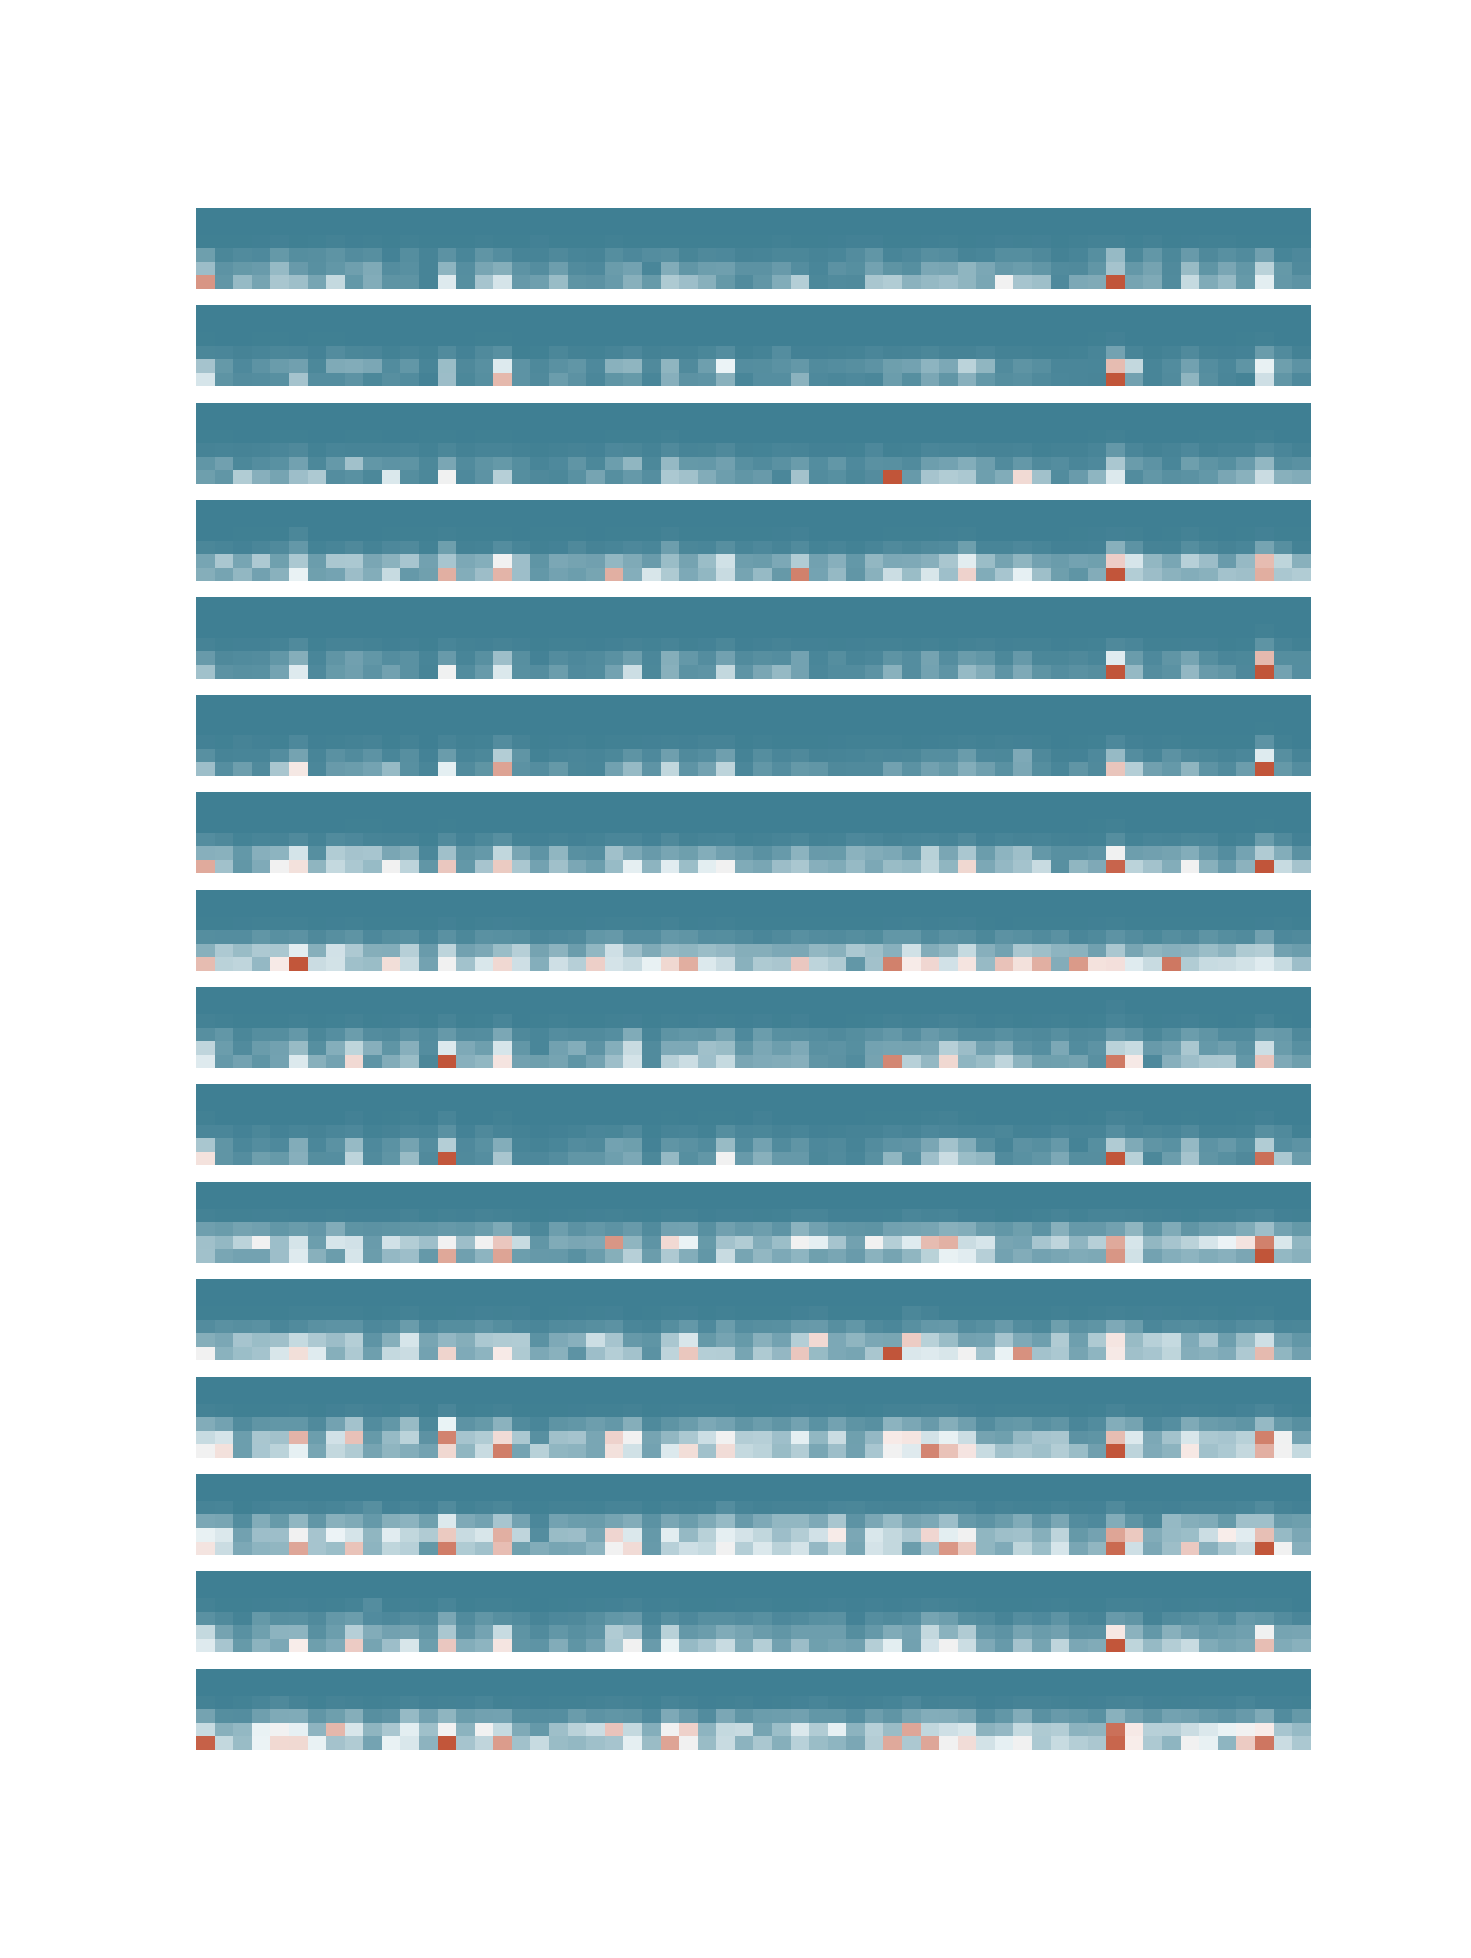
\includegraphics[scale=0.22]{img/sample_spec.eps}
    
    \column{0.5\textwidth}

    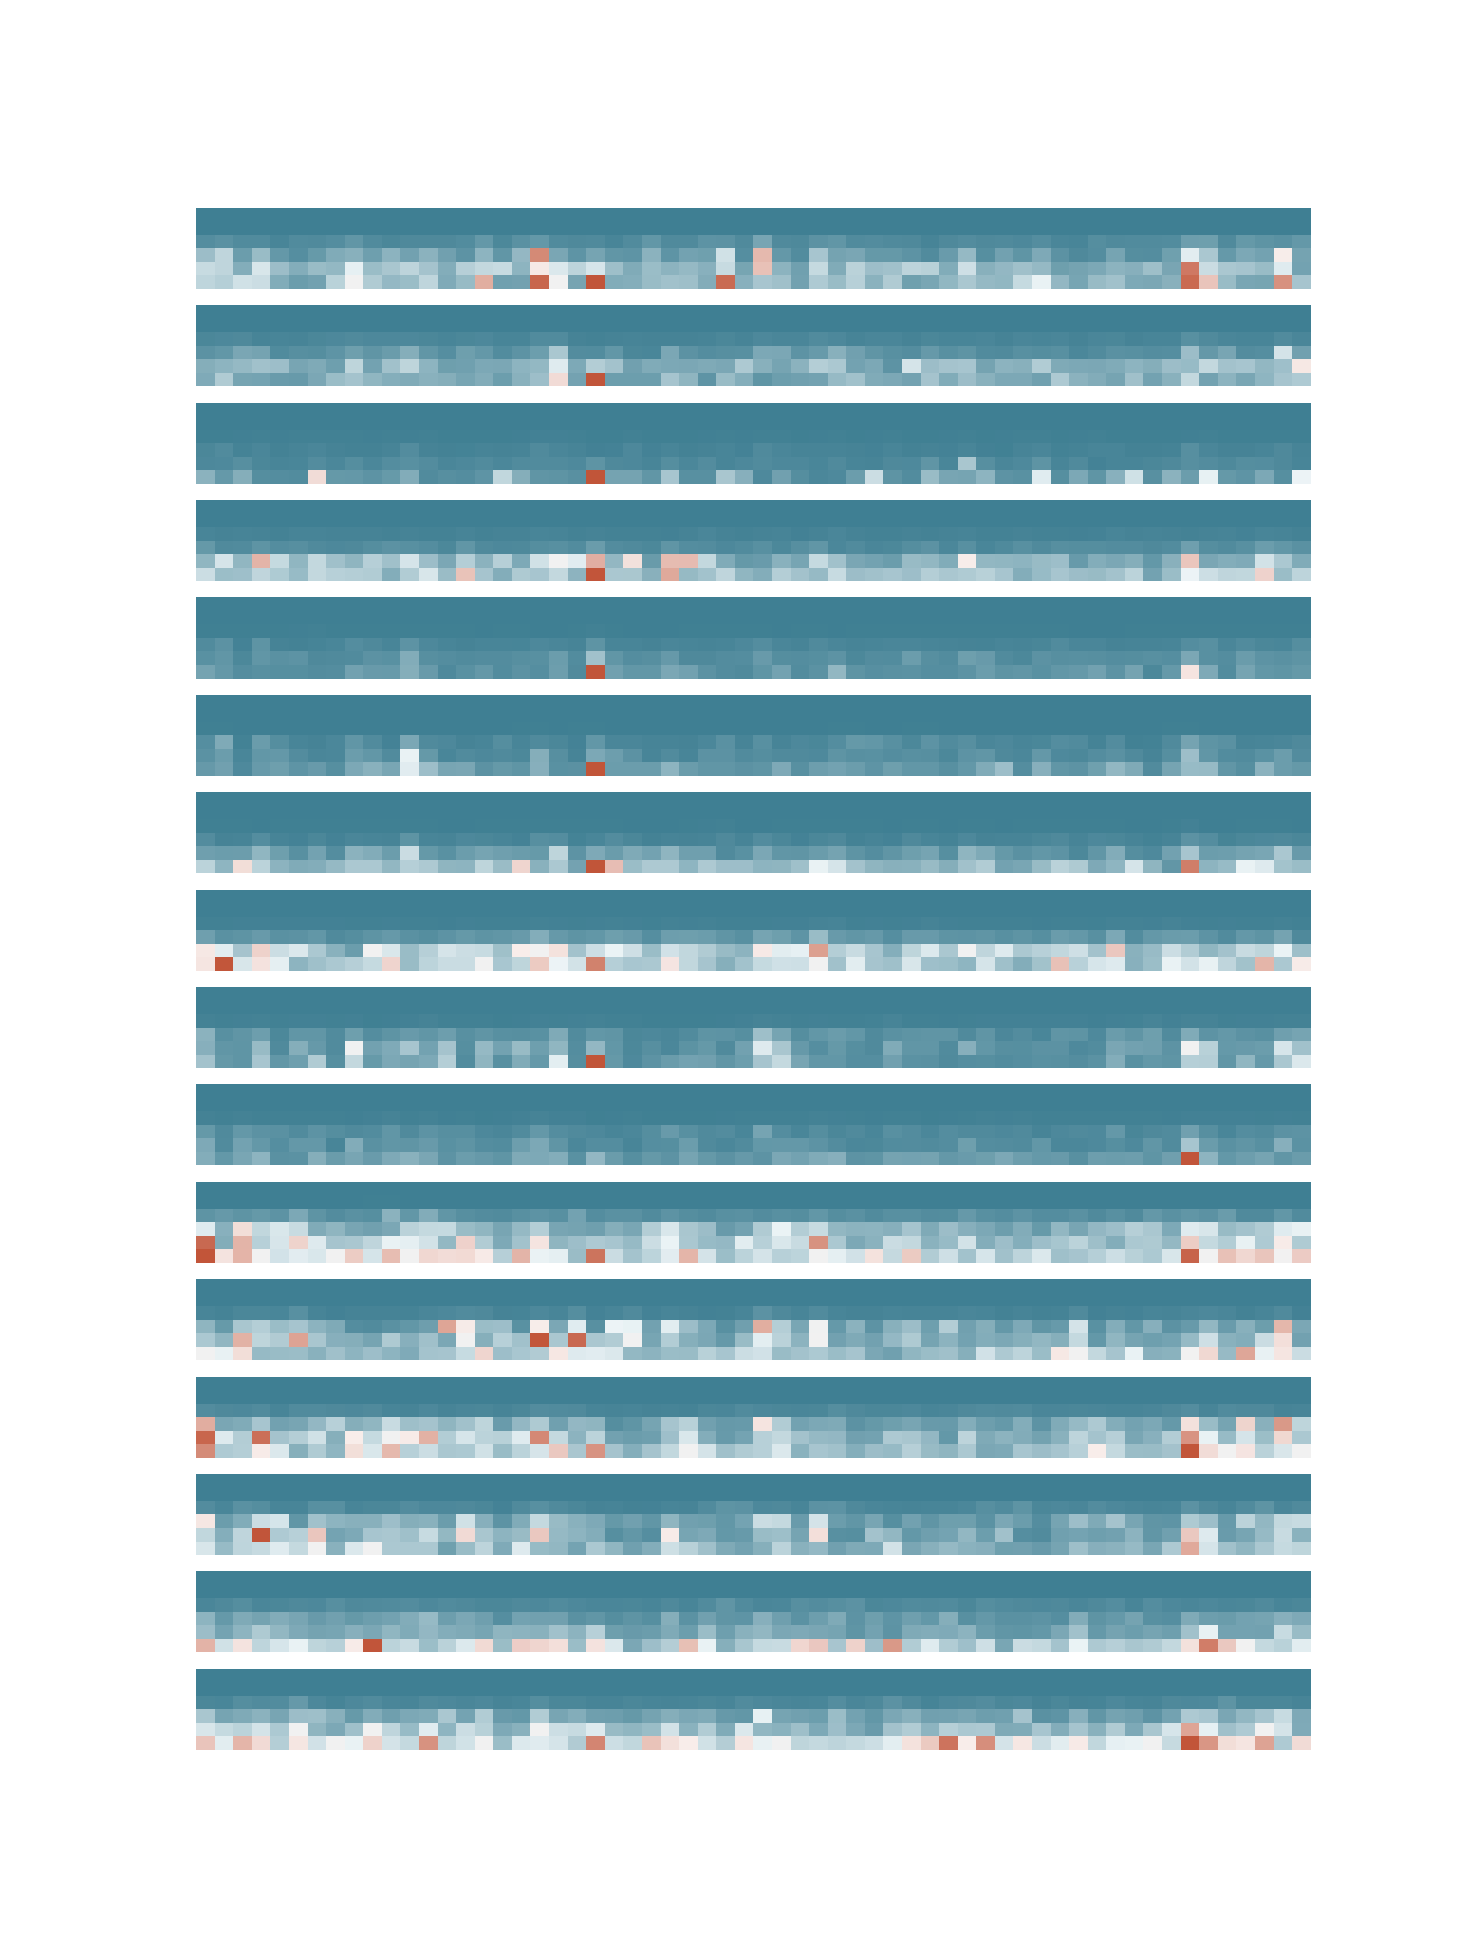
\includegraphics[scale=0.22]{img/sample_p_spec.eps}
  \end{columns}

\end{frame}


\begin{frame}{Model 1: Deep Learning (CNN) on Spectrograms}
  \framesubtitle{Overview of Convolution Neural Network (CNN)}

  \begin{block}{}
    \begin{itemize}
    \item Learns \textbf{Convolution Kernels} (more native to image operations).
    \item Apply \textbf{Pooling} to reduce dimension.
    \item Perform classification using \textbf{Dense} layers.
    \end{itemize}
  \end{block}
  
  \begin{center}
    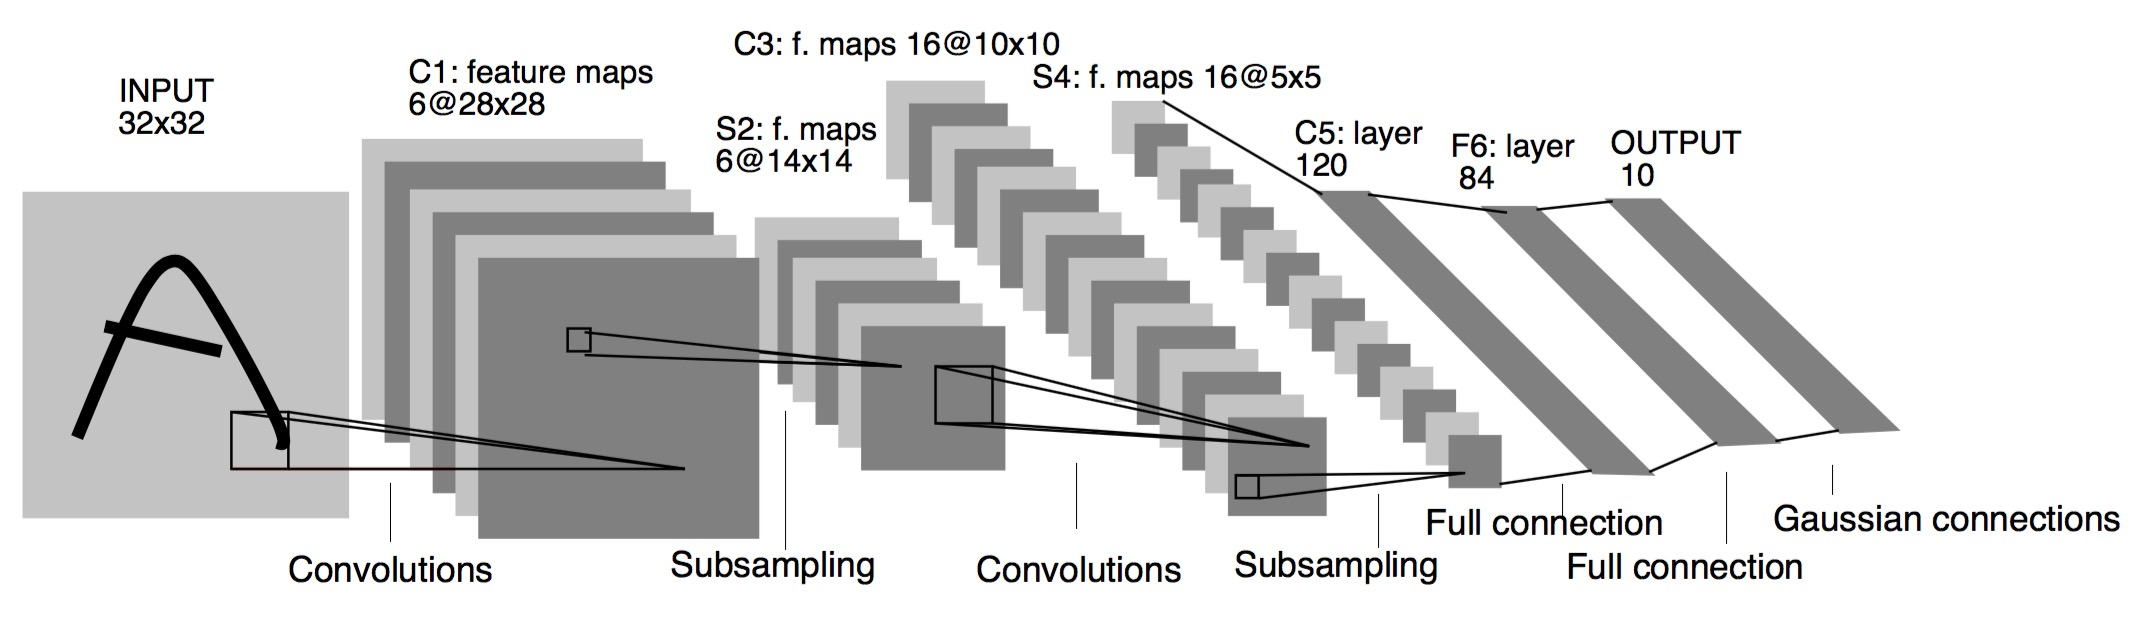
\includegraphics[scale=0.15]{img/cnn_gen.jpg}

    Ref: \texttt{https://culurciello.github.io/assets/nets/lenet5.jpg}
  \end{center}

\end{frame}



\begin{frame}{Model 1: Deep Learning (CNN) on Spectrograms}
  \framesubtitle{Overview of our CNN Architecture}
  
\end{frame}


\begin{frame}{Traditional Features Visualization}
  \framesubtitle{Fine adjustement of the watermark position}

  \begin{center}
    \vspace*{-0.15cm}
  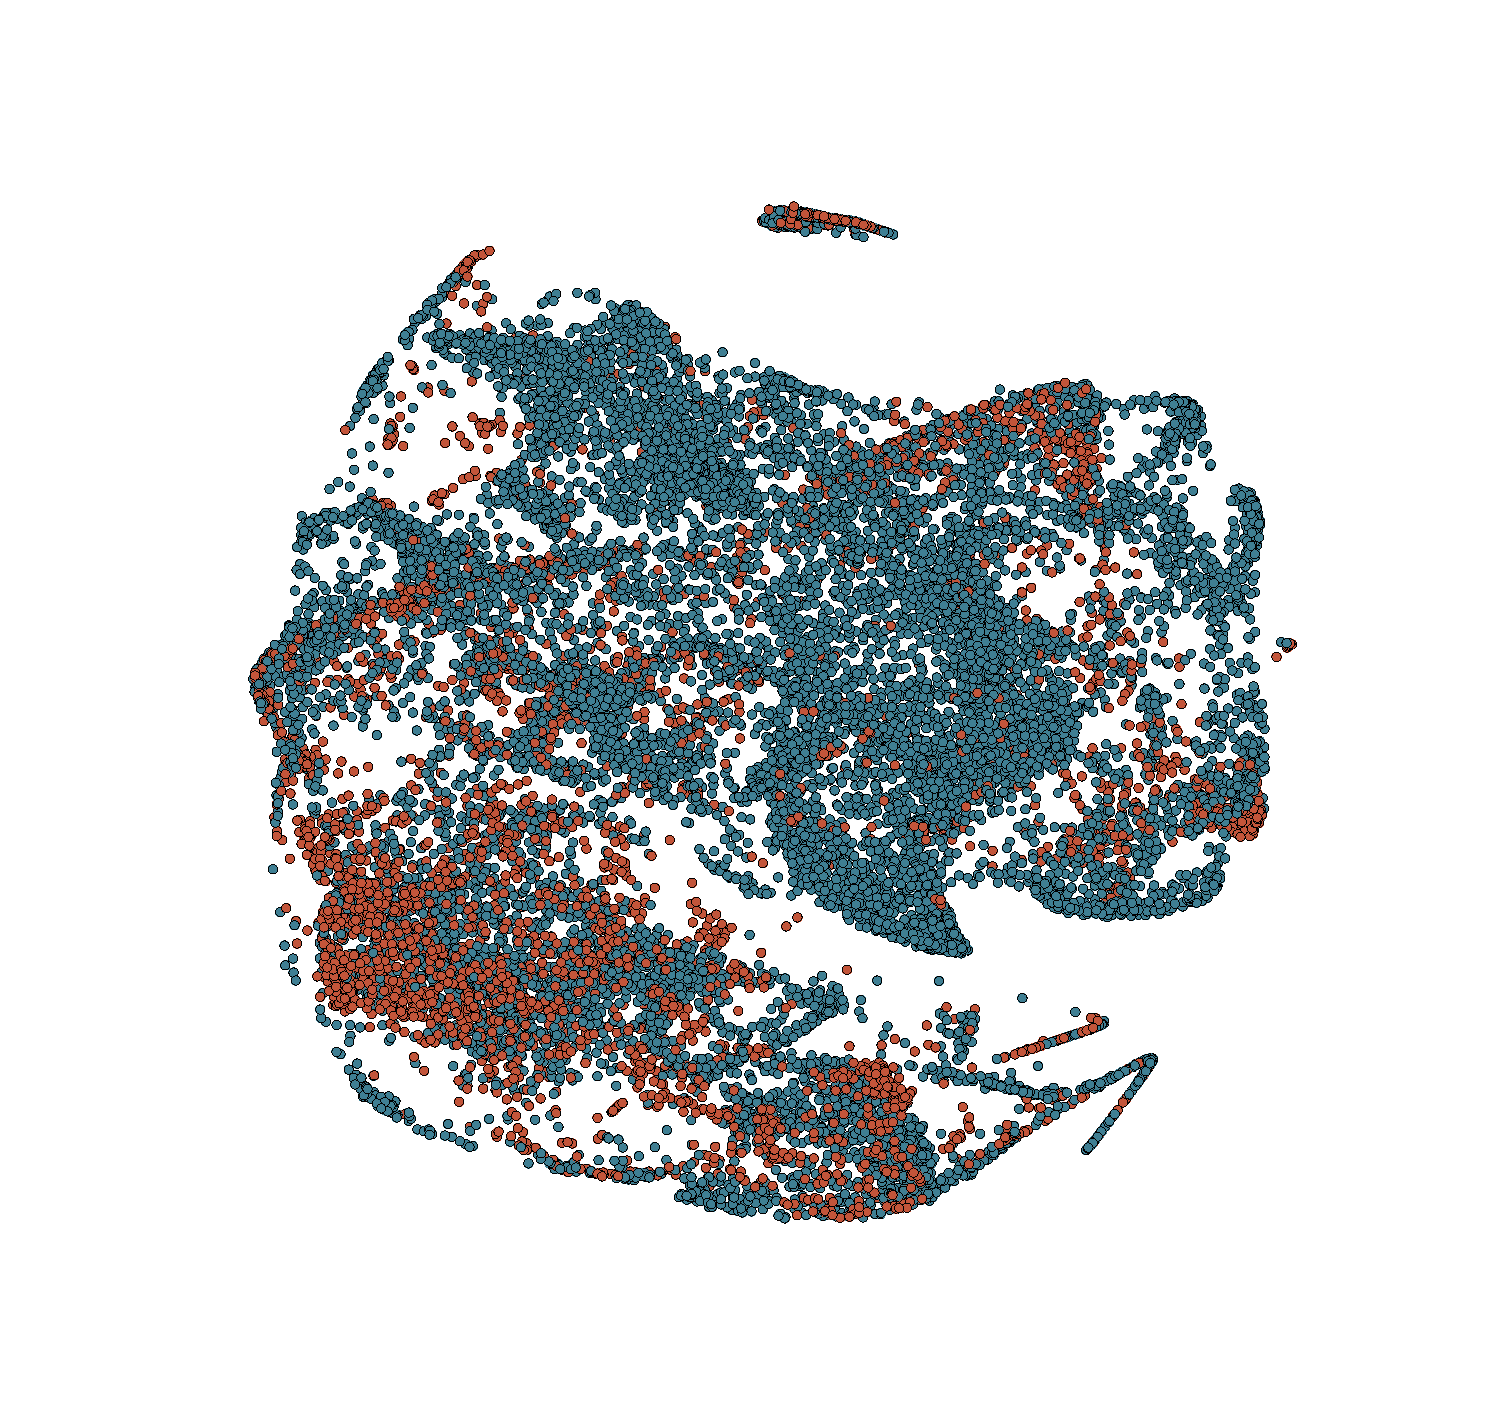
\includegraphics[scale=0.35]{img/trad_feat_viz.eps}
  \end{center}

\end{frame}


\begin{frame}{Options}
  \framesubtitle{Fine adjustement of the watermark position}

  
  \begin{itemize}
    \item \texttt{hoffset}
    \item \texttt{voffset}
  \end{itemize}
  
  They admit any \emph{positive} or \emph{negative} spacing \alert{unit}
  
  Note that some \alert{warnings} about \emph{badboxes} might be generated at compilation

\end{frame}




\begin{frame}{License}

  \begin{block}{Get the source of this theme and the demo presentation from}

  \begin{center}\url{http://github.com/famuvie/beamerthemesimple}\end{center}

  \end{block}
  
  The theme \emph{itself} is licensed under a
  \href{http://creativecommons.org/licenses/by-sa/4.0/}{Creative Commons
  Attribution-ShareAlike 4.0 International License}.

  \begin{center}\ccbysa\end{center}

\end{frame}


\bibliography{ref}
\bibliographystyle{ieeetr}

\end{document}

